
\section*{\underline{\textbf{Manual Installation of PHP}}}
Manual installation offers several benefits:
\begin{itemize}
\item Backing up, reinstalling, or moving the web server can be achieved in seconds
\item You have more control over PHP and Apache configuration. 
\end{itemize}
\subsection*{Step 1: Download the files}
Download the latest PHP 5 ZIP package from www.php.net/downloads.php\\
As always, virus scan the file and check its MD5 checksum using a tool such as fsum.
\subsection*{Step 2: Extract the files}
We will install the PHP files to C:php, so create that folder and extract the contents of the ZIP file into it.\\
PHP can be installed anywhere on your system, but you will need to change the paths referenced in the following steps.
\begin{figure}[!ht]
\centering
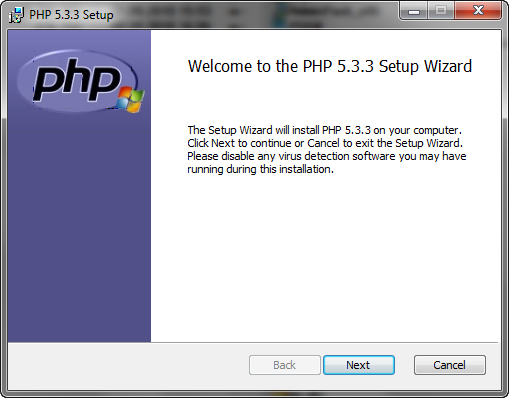
\includegraphics[width=0.6\textwidth]{/home/deepti/Desktop/10.png}                   
\caption{Installation of php}
\hspace{-1.5em}
\end{figure}
\subsection*{Step 3:Configure php.ini}
Copy C:phpphp.ini-recommended to C:phpphp.ini. There are several lines you will need to change in a text editor (use search to find the current setting).\\
Define the extension directory:\\
extensiondir = "C:phpext"\\
Enable extensions. This will depend on the libraries you want to use, but the following extensions should be suitable for the majority of applications (remove the semi-colon comment):\\
extension=phpcurl.dll\\
extension=phpgd2.dll\\
extension=phpmbstring.dll\\
extension=phpmysql.dll\\
extension=phpmysqli.dll\\
extension=phppdo.dll\\
extension=phppdomysql.dll\\
extension=phpxmlrpc.dll\\
If you want to send emails using the PHP mail() function, enter the details of an SMTP server (your ISP's server should be suitable):\\
 For Win32 only.\\
SMTP = mail.myisp.com\\
smtp port = 25\\
 For Win32 only.\\
sendmail from = my@emailaddress.com
\subsection*{Step 4: Add C:php to the path environment variable}
To ensure Windows can find PHP, you need to change the path environment variable. From the Control Panel, choose System, (then "Advanced system settings" in Vista), select the "Advanced" tab, and click the "Environment Variables" button. \\
Scroll down the System variables list and click on "Path" followed by the "Edit" button. Enter ";C:php" to the end of the Variable value line (remember the semi-colon). \\
Now OK your way out. You might need to reboot at this stage.
\subsection*{Step 5: Configure PHP as an Apache module}
Ensure Apache is not running (use "net stop Apache2.2" from the command line) and open its confhttpd.conf configuration file in an editor. The following lines should be changed:
Line 239, add index.php as a default file name:\\
DirectoryIndex index.php index.html
At the bottom of the file, add the following lines (change the PHP file locations if necessary):\\
PHP5 module\\
LoadModule php5 module "c:/php/php5apache2\textunderscore2.dll"\\
AddType application/x-httpd-php .php\\
PHPIniDir "C:/php"\\
Save the configuration file and test it from the command line (Start > Run > cmd):\\
cd Apache2bin \\
httpd -t
\subsection*{Step 6: Test a PHP file}
Create a file named index.php in Apache's web page root (either htdocs or D:WebPages) and add this code:\\
<?php phpinfo(); ?>\\
Ensure Apache has started successfully, open a web browser and enter the address http://localhost/. If all goes well, a "PHP version" page should appear showing all the configuration settings.


